There are two possible cases that results in an energy imbalance in the
detector, the first one occurs in beyond Standard Model physics, that involves
the presence of particles that interact weakly or not at all with normal
matter. These particles are not detected thus leaving an energy imbalance in the
detector. In the second case, the decay products in the final state involve
neutrinos that are not detectable by ATLAS\@. To better understand the category
category of events, consider \cref{fig:susy_standard} that shows the decay
topology of squark pair production with a neutralino and two jets in the final
state. Using the two body decay energy and momentum relations~\cite{PDG}:
\begin{equation}
  \label{eq:93}
  E_q = \frac{M_{\, \tilde{q}}^2 - m_{\, \tilde{\chi}_{\, 1}^{\, 0}}^2 + m_q^2}{2
    M_{\, \tilde{q}}},
\end{equation}
\begin{equation}
  \label{eq:94}
  |\vec{p}_q| = |\vec{p}_{\, \tilde{\chi}_{\, 1}^{\, 0}}| = \frac{\left[ \left(
        M_{\, \tilde{q}}^2 - (m_q + m_{\, \tilde{\chi}_{\, 1}^{\, 0}})^2
      \right) \left( M_{\, \tilde{q}}^2 - (m_q - m_{\, \tilde{\chi}_{\, 1}^{\,
            0}})^2 \right) \right]^{1/2}}{2 M_{\, \tilde{q}}}
\end{equation}
where $M_{\, \tilde{q}}$ is the squark center of mass energy,
$m_{\, \tilde{\chi}_{\, 1}^{\, 0}}$ is the neutralino mass and $m_q$ is the
quark mass. Neglecting the quark mass ($m_q = 0$) we get that:
\begin{equation}
  \label{eq:95}
  E_q = \frac{M_{\, \tilde{q}}^2 - m_{\, \tilde{\chi}_{\, 1}^{\, 0}}^2}{2 M_{\,
      \tilde{q}}},
\end{equation}
\begin{equation}
  \label{eq:96}
  |\vec{p}_q| = |\vec{p}_{\, \tilde{\chi}_{\, 1}^{\, 0}}| = \frac{M_{\,
      \tilde{q}}^2 - m_{\, \tilde{\chi}_{\, 1}^{\, 0}}^2}{2 M_{\, \tilde{q}}}.
\end{equation}
The quark will hadronize in the calorimeter and give rise to a jet that can be
detected by the ATLAS detector only if $\pt > 20$~GeV. If for example the mass
of the squark is $M_{\, \tilde{q}} = 450$~GeV and the mass of the neutralino is
$m_{\, \tilde{\chi}_{\, 1}^{\, 0}} = 445$~GeV then it can be seen from
\cref{eq:96} that the quark and neutralino momenta are given by
$|\vec{p}_q|~=~|\vec{p}_{\, \tilde{\chi}_{\, 1}^{\, 0}}|~\simeq~5$~GeV. Since
the neutralino escape detection, this results in low $\met$ thus when the mass
of the neutralino approaches the mass of the quark this results in a low energy
jet and $\met$ that cannot be used to trigger and select the event by the ATLAS
detector. This means that there is no sensitivity to SUSY models with compressed
mass spectra (when the mass difference between the particles is small). This
problem applies to many channels of SUSY productions.



\cref{fig:susy_exclusion} shows this effect for the search for squark pair
production in the case of the squark decaying directly to a quark and a
neutralino through the mechanism illustrated in \cref{fig:susy_standard}. This
search uses a classical multijet + $\met$ analysis, it can be seen that there is
no sensitivity close to the diagonal (dashed line) in the region
$400~<~M_{\, \tilde{q}}~<~600$~GeV.

If an initial state radiation jet is present in the event, as depicted in
\cref{fig:susy_compressed}, the squark--squark system gets boosted in the
opposite direction thus increasing the momentum of the decay products and the
missing energy leading to a signature of a high $\pt$ jet on one side and
additional jets and $\met$ on the other side of the event.

Events with an energetic jet $\pt$ and large $\met$ in the final state
constitute a clean signature for new physics searches at hadron colliders.
Signals that can be studied with this experimental signature include the
production of WIMPS, the ADD model for large extra dimensions and SUSY\@.
\begin{figure}[!h]
  \centering
  \begin{subfigure}[t]{.48\linewidth}
    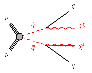
\includegraphics[width=\linewidth]{susy_standard}
    \caption{Event without initial state radiation~\cite{SUSYPub}.}
    \label{fig:susy_standard}
  \end{subfigure} \quad
  \begin{subfigure}[t]{.48\linewidth}
    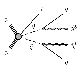
\includegraphics[width=\linewidth]{compressed}
    \caption{Event with initial state radiation~\cite{ExotPub}.}
    \label{fig:susy_compressed}
  \end{subfigure}
  \caption{Event topology of squark pair production resulting in a neutralinos
    with two jets final state with (\cref{fig:susy_compressed}) and without
    (\cref{fig:susy_standard}) initial state radiation.}
  \label{fig:motivation}
\end{figure}
\begin{figure}[!htb]
  \centering
  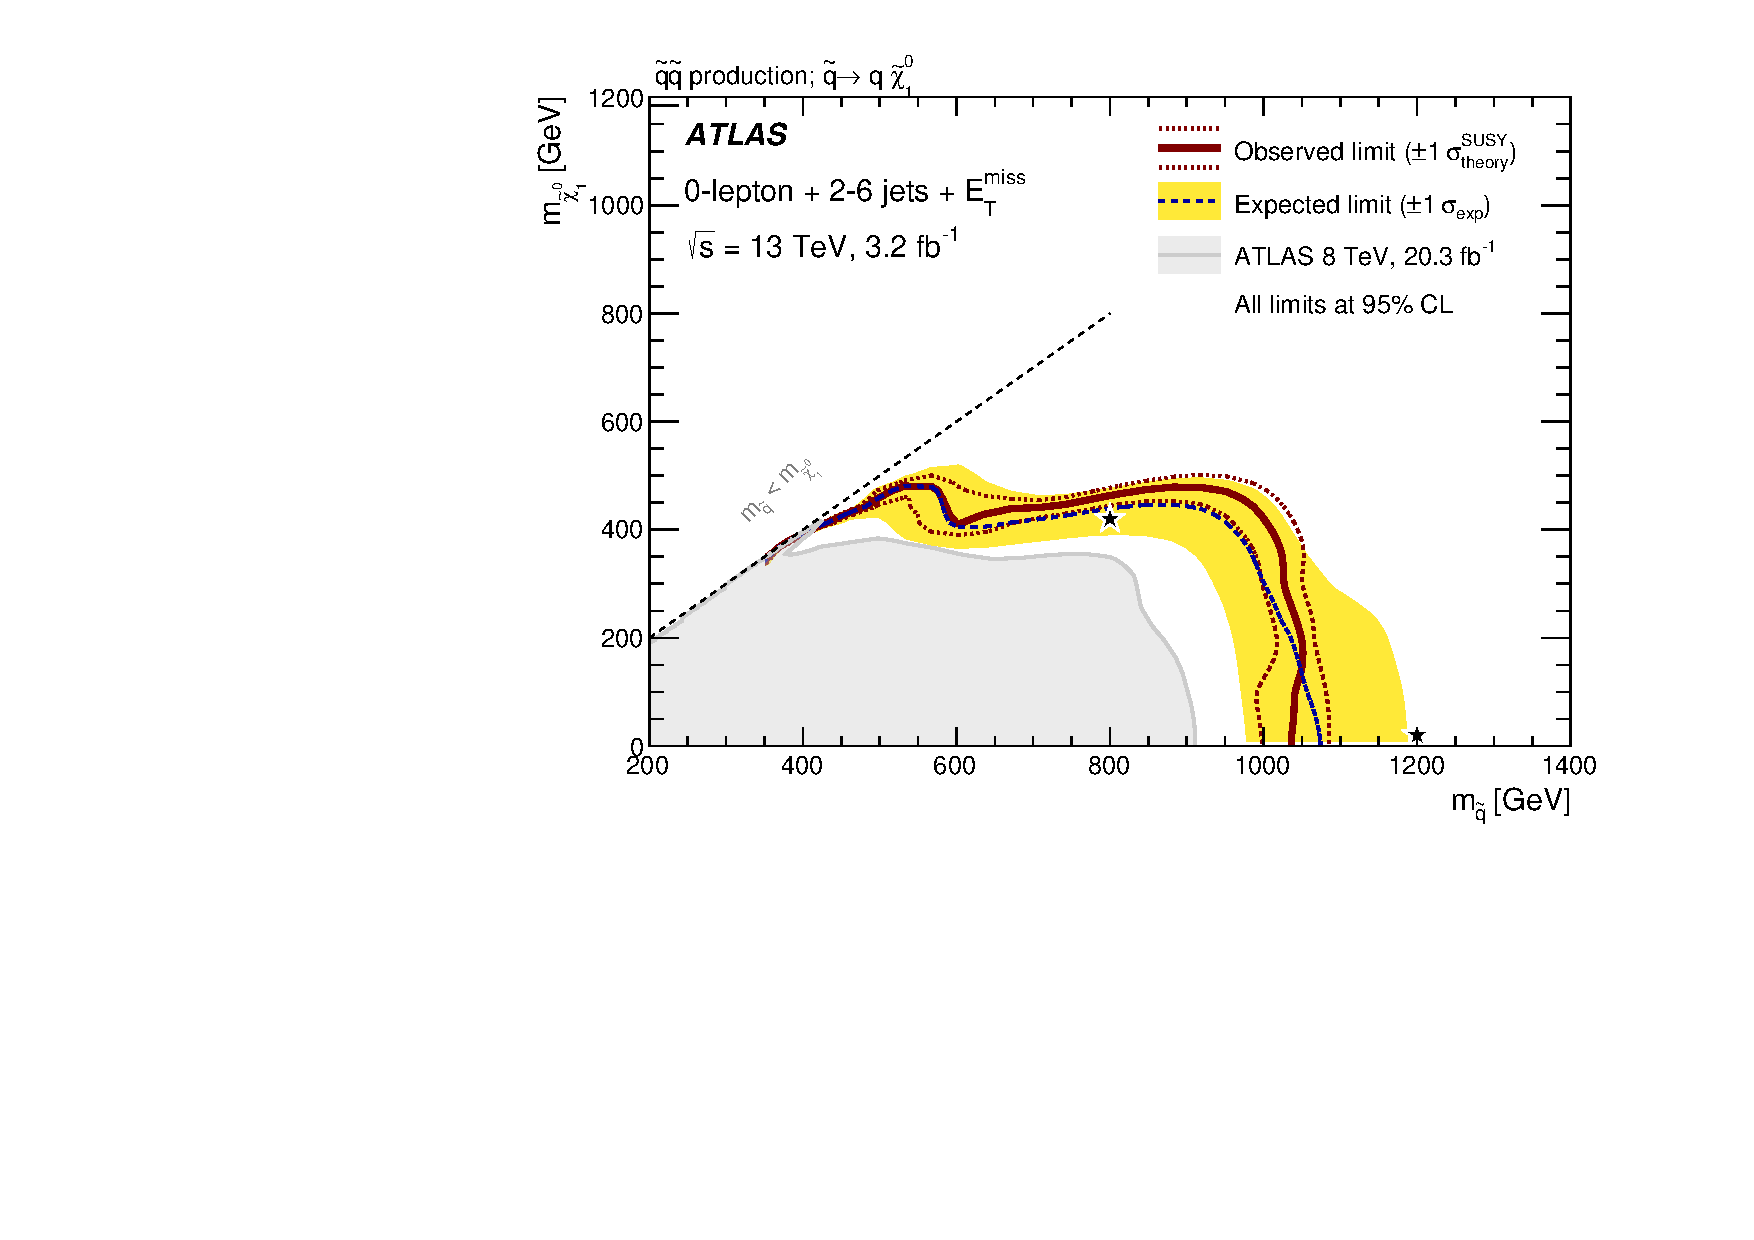
\includegraphics[width=.58\linewidth]{susy}
  \caption{Exclusion limits for direct production of squark
    pairs where the sqark decays into a quark and a neutralino. The $x$--axis
    represents the mass of the squark and the $y$--axis represents the mass of
    the lightest neutralino. The black stars represent a benchmark model as
    explained in more details in Ref.~~\cite{SUSYPub}.}
  \label{fig:susy_exclusion}
\end{figure}
%%% Local Variables:
%%% mode: latex
%%% TeX-master: "../search_for_DM_LED_with_ATLAS"
%%% End:
